\section{Incentivization Mechanism}
\label{sec:incentives}

Nodes in the HOPR network receive incentives for providing services that allow others to achieve privacy. The HOPR protocol incentivizes nodes for transforming and delivering mixnet packets. To turn this into a trustless solution, HOPR uses a custom \nameref{sec:incentives:proofofrelay} scheme which makes the nodes' work verifiable. Incentives are handled by a micropayment scheme based on \lcnameref{sec:incentives:probabilistic}. This requires the issuer of incentives to not know whether a specific incentive lead to a payout or not. The receiver of an incentive therefore deposits in advance an iterated \lcnameref{sec:incentives:commitment} to the smart contract and reveals its openings whenever claiming an incentive.

\subsection{Incentivized Behavior}
\label{sec:incentives:behavior}
\subsection{Proof of Relay}
\label{sec:incentives:proofofrelay}

The \nameref{sec:sphinx} guarantees that packets can only get processed in the order that has been chosen by the creator. As a result, after applying the required transformations, the next downstream node can either decode the packet or ends up with some random bitstring. Hence it is the next downstream node who is able to verify the correctness of the previously applied tranformations which it confirms by sending an acknowledgement.

\begin{figure}[H]
      \centering
      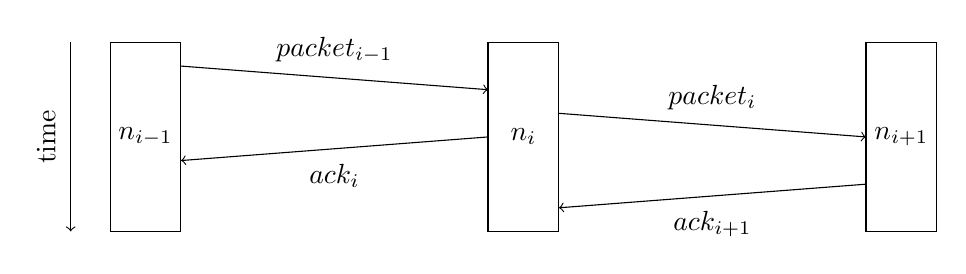
\begin{tikzpicture}
            \def\one{0.6}
            \def\nodeHeight{4*\one}
            \def\nodeWidth{1.5*\one}
            \def\nodeOffset{8*\one}

            \foreach \i\name in{0/$n_{i-1}$,1/$n_i$,2/$n_{i+1}$} {
                        \draw[shift={(\i*\nodeOffset,0)}] (0,0) rectangle (\nodeWidth,-\nodeHeight) node[midway] {\name};
                  }

            \foreach \i\packet\ack in{0/$packet_{i-1}$/$ack_i$,1/$packet_{i}$/$ack_{i+1}$} {
                        \draw[->,shift={(\i*\nodeOffset,-\i*\one)}] (\nodeWidth,-0.5*\one) -- (\nodeOffset,-\one) node[midway,above=2pt] {\packet};

                        \draw[->,shift={(\i*\nodeOffset,-\i*\one)}] (\nodeOffset,-2*\one) -- (\nodeWidth,-2.5*\one) node[midway,below=2pt] {\ack};
                  }

            \draw[->] (-0.5,0) -- (-0.5,-\nodeHeight) node[midway,left=2pt] {\rotatebox{90}{time}};
      \end{tikzpicture}
      \caption{Node $n_{i-1}$ sends $packet_{i-1}$ to node $n_i$. Node $n_i$ transforms the incoming packet, resulting in ${packet_i}$ and sends it to node $n_{i+1}$. Afterwards it acknowledges the processing of $packet_{i-1}$ to node $n_{i-1}.$}
\end{figure}

Note that acknowledgements are sent immediately once the processing of the incoming packet has been completed. This makes sure that sending acknowledgements does not create any observable pattern in reverse to the chosen path. It is rather that each acknowledgement depends on one incoming packet but it does not depend on the chosen path.

\paragraph{Construction}

Each ticket includes a challenge $C_i$ which requires a response $response_i$ to be claimable on-chain. The creator of the packet samples all of them and uses the first one for the ticket sent to the first relayer. All subsequent ones are put into the section of the routing information, see section \ref{sec:sphinx:routinginformation}, that is visible by the corresponding node. Each relayer $n_i$ and their corresponding next downstream node $n_{i+1}$ engage in a 2-out-of-2 secret sharing of $response_i$ picked by the creator of the packet. To convince each relayer that the creator of the packet knows any value $\widetilde{response_i}$ that solves $C_i$, each relayer $n_i$ receives a value $hint_i$ that serves as an argument of knowledge.

\begin{figure}[H]
      \label{fig:packetDetails}
      \centering
      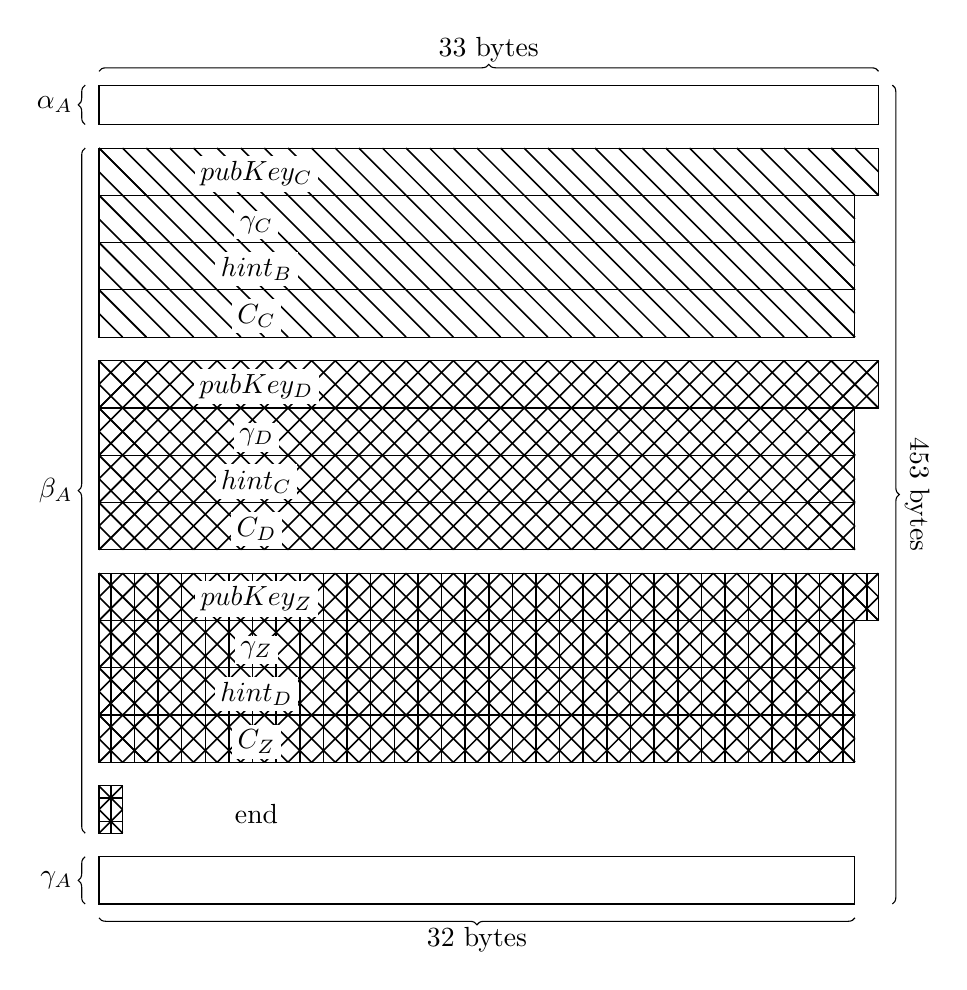
\begin{tikzpicture}
            \def\one{0.3}
            \draw[decoration={brace,raise=5pt},decorate] (0,0.5) -- node[above=5pt] {33 bytes} (33*\one,0.5);
            \draw[decoration={brace,raise=5pt},decorate] (0,0) -- node[left=6pt] {$\alpha_A$} (0,0.5) ;
            \draw[black] (0,0) rectangle (\one*33,0.5);

            \draw[decoration={brace,raise=5pt},decorate] (0,-9.0) -- node[left=6pt] {$\beta_A$} (0,-0.3);

            \foreach \name\length\offset\hatching in{$pubKey_C$/33/-0.9/1,$\gamma_C$/32/-1.5/1,$hint_B$/32/-2.1/1,$C_C$/32/-2.7/1,$pubKey_D$/33/-3.6/2,$\gamma_D$/32/-4.2/2,$hint_C$/32/-4.8/2,$C_D$/32/-5.4/2,$pubKey_Z$/33/-6.3/3,$\gamma_Z$/32/-6.9/3,$hint_D$/32/-7.5/3,$C_Z$/32/-8.1/3}{
                        \draw (0,\offset) rectangle (\one*\length,\offset+0.6);
                        \begin{scope}[shift={(0,\offset)}]
                              \ifnum\length=33
                                    \def\a{9.9}
                                    \def\diff{9.4}
                              \else
                                    \def\a{9.6}
                                    \def\diff{9.1}
                              \fi
                              \def\b{0.6}
                              \def\lw{0.2}

                              \foreach \x [count=\i] in{0,0.3,0.6,...,\b}{
                                          \draw [line width=\lw mm](\x,0)--(0,\x) (\a-\b+\x,\b)--(\a,\x);
                                    }
                              \foreach \x [count=\i] in{0,0.3,0.6,...,\diff}{
                                          \draw [line width=\lw mm](\x+\b,0)--(\x,\b);
                                    }

                              \ifnum\hatching>1
                                    \foreach \x [count=\i] in{0,0.3,0.6,...,\b}{
                                                \draw [line width=\lw mm](0,\x)--(\b-\x,\b) (\a-\b+\x,0)--(\a,\b-\x);
                                          }
                                    \foreach \x [count=\i] in{0,0.3,0.6,...,\diff}{
                                                \draw [line width=\lw mm](\x,0)--(\b+\x,\b);
                                          }
                              \fi

                              \ifnum\hatching>2
                                    \foreach \x [count=\i] in{0,0.15,0.45,...,\a}{
                                                \draw [line width=\lw mm](\x,0)--(\x,\b);
                                          }
                              \fi
                        \end{scope}

                        \draw (2.0,\offset+0.25) node[fill=white,above=-6pt,inner sep=2pt] {\name};
                  }

            \draw (0,-8.4) rectangle (\one*1,-9.0);

            \begin{scope}[shift={(0,-9.0)}]
                  \def\lw{0.2}

                  \draw [line width=\lw mm](0,0)--(0.3,0.3);
                  \draw [line width=\lw mm](0,0.3)--(0.3,0.6);

                  \draw [line width=\lw mm](0,0.6)--(0.3,0.3);
                  \draw [line width=\lw mm](0,0.3)--(0.3,0);

                  \draw [line width=\lw mm](0.15,0)--(0.15,0.6);

                  \draw [line width=\lw mm](0,0.15)--(0.3,0.15);
                  \draw [line width=\lw mm](0,0.45)--(0.3,0.45);

                  \draw (2.0,0.25) node[fill=white,above=-7pt] {end};
            \end{scope}

            \draw[decoration={brace,raise=5pt},decorate] (0,-9.9) -- node[left=6pt] {$\gamma_A$} (0,-9.3);

            \draw (0,-9.3) rectangle (\one*32,-9.9);
            \draw[decoration={brace,mirror,raise=5pt},decorate] (0,-9.9) -- node[below=5pt] {32 bytes} (32*\one,-9.9);

            \draw[decoration={brace,raise=5pt},decorate] (33*\one,0.5) -- node[midway,right=6pt] {\rotatebox{270}{453 bytes}} (33*\one,-9.9) ;

      \end{tikzpicture}
      \caption{Mixnet packet header with PoR fields that is sent from the sender $A$ to $B$ and supposed to be forwarded through nodes $C, D$ to $Z$.}
\end{figure}

\paragraph{Secret sharing}
\label{sec:incentives:proofofrelay:secretSharing}

Each node derives two keys, $s_i^{own}$ and $s_i^{ack}$, by using the $s_i$ as given by the SPHINX packet (see the \lcnameref{appendix:keyderivation} section for more details). $s_i^{own}$ and $s_{i+1}^{ack}$ serve as key shares of a 2-out-of-2 secret sharing between a node $n_i$ and the next downstream node $n_{i+1}$ along the chosen path. Once a node knows \textit{both} key shares, $s_i^{own}$ and $s_{i+1}^{ack}$, it is able to reconstruct $s_i^{response}$ to redeem the received ticket on-chain.

Whilst $s_i^{own}$ is derivable upon reception of a packet, $s_{i+1}^{ack}$ requires the cooperation of the next downstream node $n_{i+1}$ and is sent as an \textit{acknowledgement} if $n_{i+1}$ has received the transformed packet and considers both the packet and embedded ticket valid.

\begin{figure}[H]
      \centering
      \begin{tikzpicture}[auto]
            \draw (0,0) node (a) {};
            \draw (3.0,0) node (b) [rectangle,draw] {$n_{i-1}$};
            \draw (6,0) node (c) [rectangle,draw] {$n_i$};
            \draw (9.0,0) node (d) [rectangle,draw] {$n_{i+1}$};
            \draw (12.0,0) node (e) {};

            \draw (6.0, -1.5) node [circle,draw] (intermediateResult) {};
            \draw (6.0, -2.5) node (response) {$s_i^{response}$};

            \draw [->,draw,dashed] (a.east) to node [align=center,below] {packet$_{i-2}$} (b.west);
            \draw [->,draw,dashed] (b.east) to node [align=center,below] {packet$_{i-1}$} node [align=center,above,circle] {\color{hopr-blue}1.} (c.west);
            \draw [->,draw,dashed] (c.east) to node [align=center,below] {packet$_i$} node [align=center,above,circle] {\color{hopr-blue}2.} (d.west);
            \draw [->,draw,dashed] (d.east) to node [align=center,below] {packet$_{i+1}$} (e.west);

            \draw [->,draw] (c.south) to node [right] {$s_i^{own}$} node [align=center,left=1pt,circle] {\color{hopr-blue}3.}  (intermediateResult.north);
            \draw [->,draw,bend left] (d.south) to node[below] {$s_{i+1}^{ack}$} node [align=center,right=5pt,circle] {\color{hopr-blue}4.} (intermediateResult.east);
            \draw [->,draw] (intermediateResult.south) to (response.north);
      \end{tikzpicture}
      \caption{\color{hopr-blue}1. \color{black} Node $n_i$ receives $packet_{i-1}$, validates it, transforms it and \color{hopr-blue}2. \color{black} sends it to node $n_{i+1}$. \color{hopr-blue}3. \color{black} While processing $packet_i$, node $n_i$ derives $s_i^{own}$ and \color{hopr-blue}1. \color{black} once node $n_{i+1}$ considers $packet_i$ valid, it \textit{acknowledges} the receipt of $packet_i$ and thereby reveals $s_{i+1}^{ack}$ to node $n_i$ which allows node $n_i$ to reconstruct $s_i^{response}$.}
      \label{fig:proofofrelay}
\end{figure}

\paragraph{Challenge response}

Tickets sent next to a mixnet packet include a challenge $C_i$ which is computed as $$C_i = s_i^{response} \cdot G = (s_i^{own} + s_{i+1}^{ack}) \cdot G$$ where $G$ refers to the base point and $\cdot$ means scalar multiplication on the curve. Hence, in order to solve the challenge, it is necessary to know $s_i^{own}$ as well as $s_{i+1}^{ack}$.

\paragraph{Challenge and Hint}
\label{sec:incentives:proofofrelay:challenge}

Once a node receives a packet, it is able to derive $s_i^{own}$ but it is unable to decide whether $s_{i+i}^{ack}$ will ever lead to $s_i^{response}$ that solves the challenge. Since the underlying field preserves the distributivity, it holds that $$C_i = s_i^{response} \cdot G = (s_i^{own} + s_{i+1}^{ack}) \cdot G = s_i^{own} \cdot G + s_{i+1}^{ack} \cdot G$$

Hence by knowing $hint_i = s_{i+1}^{ack} \cdot G$, the node can verify that $s_i^{own} \cdot G + hint_i = C_i$ and thereby check that the creator of the challenge must have known a value $\tilde{s}_{i+1}^{ack}$ that led to $hint_i$. Due to the infeasibility of inverting scalar multiplication on the chosen curve, knowing $hint_i$ does not reveal $s_{i+1}^{ack}$. Hence, by embedding $hint_i$ into the part of $\beta$ within the SPHINX packet that is readable by node $n_i$, the sender makes the validity of the embedded challenge verifiable.

As the next downstream node would not accept a packet without a ticket\footnote{By default, nodes only forward packets that include incentives. Nevertheless, the protocol does not prevent them from processing packets without enforcing an incentive.}, the node $n_i$ not only needs to transform the packet but must also issue a ticket to the next downstream node $n_{i+1}$. Therefore, it needs to know which challenge $\tilde{C}_{i+1}$ to put into the ticket issued for node $n_{i+1}$. As in the previous section, this is done with the help of the creator of the packet, who embeds $C_{i+1}$ into the part of the SPHINX packet that is readable by node $n_{i+1}$.

By chaining this principle, nodes are forced to \textit{always} issue a ticket to the next downstream node because they are unable to claim their own incentive without the help of the next downstream node.

Since the very last node, namely the final recipient, of the packet, does not need to forward the packet to anyone else, it has no direct incentive to acknowledge tickets, hence there are no direct consequences for not acknowledging packet. In its current version, the protocol does not prevent this kind of behaviour, but research is being conducted into the necessity and feasibility of solving this issue via a reputation system.
\subsection{Probabilistic Payment Channels}
\label{sec:incentives:probabilistic}

Payment channels give two nodes, $A$ and $B$, the opportunity to lock funds on-chain and later on handle who of them possesses which fraction. At each moment, it holds that

$$ balance(A) + balance(B) = const. $$

The state becomes final once one of the nodes submits the most recent state to the smart contract. Therefore it requires a proof by the counterparty that the proclaimed state is in their interest, which is given by a digital signature and named \textit{update transaction}. Hence an update transaction that transfers $x > 0$ digital assets from $A$ to $B$ is approved by,

$$ update_i = Sig_A (balance(A) - x \ || \ balance(B) + x) $$

By doing so, payments can only in one direction, turning the payment channel into a unidirectional payment channel. This is possible because digital assets will only be transferred from $A$ to $B$ and thus $B$ will always pick in its own the interest the most recent update transaction since $balance(B)$ is strictly increasing.

If the channel allowed asset transfers in the opposite direction, namely from $B$ to $A$ the update transactions need to include a versioning element that prevents any of the parties from rollback to the most beneficial state since the smart contract is unable to determine the most recent transaction otherwise. Hence,

$$ update_i = Sig_A (i \ || \ balance(A) - x \ || \ balance(B) + x) $$

In addition, this requires certain timeframes in which the counterparty is given the opportunity to present their most recent update update transaction. This is necessary because none of the nodes can prove that there does \textit{not} exist a more recent update transaction. Once the timeout ends, and none of the parties have submitted any more recent update transaction, the last submitted state becomes final.

\begin{figure}[H]
    \centering
    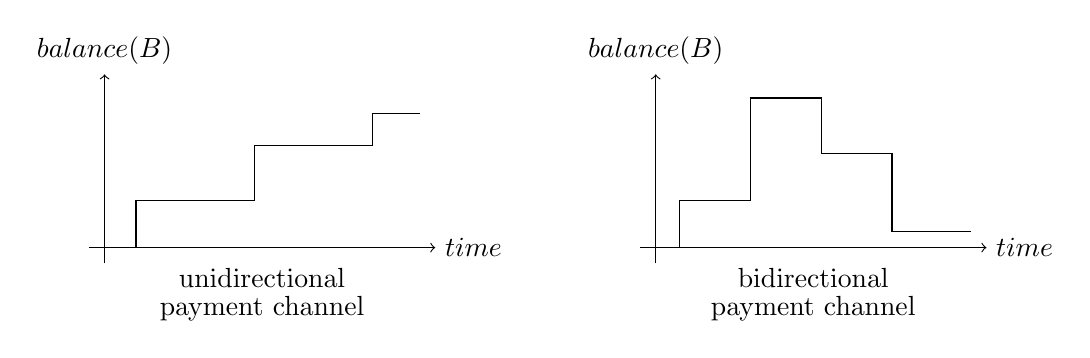
\begin{tikzpicture}[domain=0:2]
        \def\padding{0.1}
        \def\plotHeight{2}
        \def\plotWidth{4}
        \def\plotOffset{7}
        \def\textOffset{0.6}
        \foreach \i in {0,1} {
                \begin{scope}[shift={(\i*\plotOffset,0)}]
                    \draw[->] (-2*\padding,0) -- (\plotWidth+2*\padding,0) node[right] {$time$};
                    \draw[->] (0,-2*\padding) -- (0,\plotHeight+2*\padding) node[above] {$balance(B)$};

                    \ifnum\i=0
                        \path (0,-\textOffset) -- (\plotWidth,-\textOffset) node[midway] {\shortstack{unidirectional\\payment channel}};
                        \draw (0.4,0) -- (0.4,0.6) -- (1.4,0.6) -- (1.9,0.6) -- (1.9,1.3) -- (2.6,1.3) -- (3.4,1.3) -- (3.4,1.7) -- (4.0,1.7);
                    \else
                        \path (0,-\textOffset) -- (\plotWidth,-\textOffset) node[midway] {\shortstack{bidirectional\\payment channel}};

                        \draw (0.3,0) -- (0.3,0.6) -- (1.2,0.6) -- (1.2,1.9) -- (2.1,1.9) -- (2.1,1.2) -- (3.0,1.2) -- (3.0,0.2) -- (4.0,0.2);
                    \fi
                \end{scope}
            }
    \end{tikzpicture}
    \label{fig:channels}
    \caption{Node $A$ and $B$ have a payment channel. Whilst in case of unidirectional payment channels, $balance(B)$ is strictly increasing, the derivative of $balance(B)$ \textit{can} change sign if the channel is bidirectional.}
\end{figure}

Within the HOPR protocol, payment channels are implemented as unidirectional channels, hence there \textit{can} be one from $A \rightarrow B$ and another one from $B \rightarrow A$. Whenever, an update transaction is submitted to the blockchain, the assets get transferred to the channel in the opposite direction, or directly to the counterparty if there is no such channel. This obviously controverses the original purpose of payment channels, which is \textit{aggregation} of asset transfers.

When talking about unidirectional payment channels, aggregation means that $value(update_i) = value(update_{i-1}) + \Delta x$, hence $update_i$ makes $update_{i-1}$ obsolete as it already includes the additional assets $\Delta x$. So, if a node manages to receive $update_i$ before $update_{i-1}$, there is no need to provide the services the which were supposed to be compensated by $update_{i-1}$.

This is problematic for HOPR because it uses \nameref{sec:incentives:proofofrelay} to unlock payment made from one node to the other and the state of a payment channel between nodes $n_{i-1}$ and $n_i$ therefore relies on third-party actions, namely by $n_{i+1}$ and $n_{i+1}'$. Both of them acknowledge the reception of the packet and the correct transformation done by node $n_i$. Using update transactions arises the question which update transaction node $n_{i+1}$ and node $n_{i+1}'$ should sign because they cannot know which acknowledgement reaches $n_i$ first. Hence, the incentives for packet need to be done independently and thus should not rely on update transactions.

\begin{figure}[H]
    \centering
    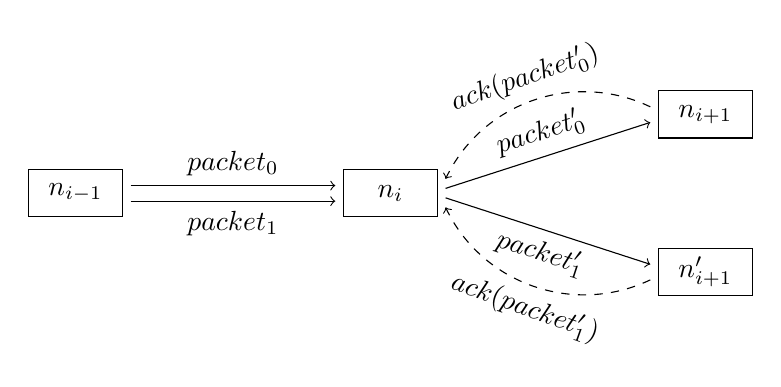
\begin{tikzpicture}
        \def\nodeOffset{4}
        \def\nodeYOffset{1}
        \def\nodeWidth{1.2}
        \def\nodeHeight{0.6}
        \def\padding{0.1}

        \foreach \xOffset\yOffset\name in{-\nodeOffset/0/$n_{i-1}$,0/0/$n_i$,\nodeOffset/\nodeYOffset/$n_{i+1}$,\nodeOffset/-\nodeYOffset/$n_{i+1}'$} {
                \draw[shift={(\xOffset,\yOffset)}] (0,0) rectangle (\nodeWidth,\nodeHeight) node[midway] {\name};
            }

        % Packets
        \draw[->,shift={(0,0.66*\nodeHeight)}] (-\nodeOffset+\nodeWidth+\padding,0) -- (-\padding,0) node[midway,above] {$packet_0$};
        \draw[->,shift={(0,0.33*\nodeHeight)}] (-\nodeOffset+\nodeWidth+\padding,0) -- (-\padding,0) node[midway,below] {$packet_1$};

        % Forwarded packets
        \draw[->] (\nodeWidth+\padding,0.6*\nodeHeight) -- (\nodeOffset-\padding,\nodeYOffset+0.33*\nodeHeight) node[midway,sloped,above] {$packet_0'$};
        \draw[->] (\nodeWidth+\padding,0.4*\nodeHeight) -- (\nodeOffset-\padding,-\nodeYOffset+0.66*\nodeHeight) node[midway,sloped,below] {$packet_1'$};

        % Acknowledgements
        \draw[->,dashed] (\nodeOffset-\padding,\nodeYOffset+0.66*\nodeHeight) to [bend right=45] node[above,sloped] {$ack(packet_0')$} (\nodeWidth+\padding,0.8*\nodeHeight);
        \draw[->,dashed] (\nodeOffset-\padding,-\nodeYOffset+0.33*\nodeHeight) to [bend left=45] node[below,sloped] {$ack(packet_1')$} (\nodeWidth+\padding,0.2*\nodeHeight);
    \end{tikzpicture}
    \caption{Node $n_{i-1}$ send packet $packet_0$, $packet_1$ to node $n_i$ which forwards them to node $n_{i+1}$ and node $n_{i+1}'$. Both nodes acknowledge the validity of $packet_0'$ and $packet_1'$ to node $n_i$.}
    \label{fig:sharedpaymentchannel}
\end{figure}

\paragraph{Probabilistic payments}
\label{sec:incentives:probabilistic:probabilistic}

Incentives relate to packets which are assumed to be sent very often in the HOPR network. Nodes can therefore expect that they will shortly receive another micropayment from the same node. It is thus not necessary to claim the incentive for each packet individually. This is why nodes issue each other probabilistic \lcnameref{sec:tickets} that have the same asymptotic payout but do neither require in-order processing nor require an on-chain operation for every incentive. Hence when picking the same relay fee, it holds that

$$ \forall i \ \forall j \ : \ value(ticket_i) = value(ticket_j) $$

Moreover, the nodes estimate the usage of the link to the nodes with whom they have engaged in a payment channel and pick a ticket winning probability that leads to a continous payout. Connections with higher througput can use lower probabilities whilst those with fewer traffic are supposed to use winning probabilities closer to 1.

Probabilistic payments rely on the necessity for the ticket issuer to not know whether a ticket that is issued will turn into an asset transfer or not. Hence, the ticket redemption must rely on some entropy provided by the ticket redeemer and need to be kept secret until the ticket is redeemed. This is necessary, because by knowing which ticket is going to become a winner, the ticket issuer would solely issue losing tickets and thereby withhold the incentives for the next downstream node.

Analogously, the ticket receiver should not know whether a ticket will be a win before being able to reconstruct the response to the challenge stated in the ticket. If not, the ticket receiver would just process those packet that come with a winning ticket and drop all other packets.

A ticket is a winner if

$$ keccak256 ( ticketHash \ || \ porSecret \ || \ opening) < ticket.invWinProb $$

where $ticketHash$ is the hash of the received ticket, see section \ref{sec:tickets:redemption}, and thus known by both ticket issuer and recipient whereas $porSecret$ is known by the ticket issuer and can be reconstructed as part of the $\nameref{sec:incentives:proofofrelay}$ scheme by the ticket recipient once it receives the acknowledgement for the forwarded ticket. On the other hand, $opening$ refers to the value that opens the most recent commitment that is stored on-chain, see section \ref{sec:incentives:commitment}. The on-chain commitment is chosen by the ticket recipient and due to the hiding property of the utilized commitment scheme, the opening values are solely known by the ticket recipient.
\subsection{On-chain Commitment}
\label{sec:incentives:commitment}

As seen in previous section \ref{sec:incentives:probabilistic}, ticket luck relies on two sources of entropy, one provided by the ticket issuer and one provided by the recipient. This section focuses on the entropy provided by the ticket recipient.

The entropy need be kept hidden until the ticket gets redeemed. In addition, the ticket recipient must not be able to change the entropy just before redeeming a ticket turn previously losing tickets into winners. Furthermore, as redeeming the ticket reveals the entropy and thus loses its value, it need to be reset with every ticket redemption. Last but not least, the mechanism must be feasible to implement it within Ethereum.

To match the aforementioned properties, HOPR uses an iterated on-chain commitment scheme that is initialized once the channel is opened. The scheme is iterative, so by revealing a commitment, the ticket recipient sets the upcoming commitment and the smart contract keeps this value for the next ticket redemption.

\paragraph{Commitment scheme}
\label{sec:incentives:commitment:scheme}

The commitment scheme in HOPR is a tuple of three algorithms, $(\mathsf{KeyGen}, \mathsf{Commit}, \mathsf{Open})$. \textsf{KeyGen} takes a security parameter and returns a seed $x$. \textsf{Commit} takes $x$ and produces the commitment as $ cm = Commit(x) $. \textsf{Open} takes a commitment $cm$ and $r$ and fails if $x$ does not fit to $cm$, otherwise it return $1$.

The commitment scheme is called binding if it is infeasible for an adversary to find a value $x' \ne x$ such that $\mathsf{Open}(cm, x') = 1$. It is called hiding if is infeasible for an adversary to derive the commited value $x$ from $cm$.

The iterated commitment scheme is computed as

$$ comm_i = keccak256 ^i (x) = keccak256 ^{i-1} (keccak256 (x)) \quad \text{for} \ i > 0$$

where $comm_0 = x$ and thus servers as a master secret. The value $x$ is chosen randomly by the ticket recipient, hence due to the pseudorandomness of the utilized cryptographic hash function, for every $i > 0$, the resulting value $comm_i = keccak256(comm_{i-1})$ is pseudorandom as well and therefore infeasible to predict by the ticket issuer.

The algorithm \textsf{Open} is therefore quite simple as it solely checks that

$$ comm_i = keccak256 (\widetilde{comm_{i-1}}) $$

\paragraph{Commitment phase}
\label{sec:incentives:commitment:commitmentphase}

Once a node is the destination of a payment channel, it samples a master key $comm_0 \in \{ 0, 1\} ^32$ and computes $comm_n = keccak256^n(comm_0)$ and submits a transaction that stores $comm_n$ on-chain within the payment channel. The value $n > 0$ is chosen by the ticket recipient and should reflect the amount of tickets that are expected to be sent using this channel.

Obviously, the ticket recipient can run out of openings after redeeming a huge amount of tickets - or losing the master secret $x$. Therefore, the ticket recipient has the opportunity to renew the stored on-chain commitment. As this would allow the recipient to alter the opening to a more pleasant value just before redeeming a ticket, i.e. to turn a previously losing ticket into a winning one. Therefore, each payment channel includes a counter that gets increased on every renewal.

$$ channel.ticketEpoch = channel.ticketEpoch + 1 $$

Increasing that counter invalidates all previously issued tickets, hence there is no incentive for the ticket recipient to renew it more than necessary.

\paragraph{Opening phase}

In order to redeem a ticket, the ticket recipient must reveal the opening $comm_{i-1}$ to the current commitment $comm_i$ stored within the smart contract.

The smart contract therefore checks that

$$ channel.commitment = keccak256 (\widetilde{comm_{i-1}}) $$

If the values match, the smart contract sets $channel.commitment = comm_{i-1}$, hence the ticket recipient needs to reveal $comm_{i-2}$ to redeem the next ticket.

\subsection{Payment Channel Management}
\label{sec:incentives:channels}

Sending a packet requires the node $n_{open}$ to issue a ticket to the next downstream node $n_{dest}$ which cannot be done without an open payment channel towards $n_{dest}$. So, in order to send a packet, the $n_{open}$ first needs open a payment channel and thereby deposit assets to cover for upcoming tickets that will be issued towards $n_{dest}$.

A payment channel runs throug multiple states during its lifecycle: Initially, each payment channel is \textit{Closed}. Node $n_{open}$ can create one by locking some assets in the smart contract, which leads to \textit{WaitinForCommitment}. This step is necessary because the payment channel becomes usable once $n_{dest}$ has set a commitment. Once that is done, a payment channel is considered \textit{Open}. If the counterparty has already set commitment, then funding immediately changes the state to \textit{Open}. As long as a payment channel is open, the counterparty can submit ticket to redeem them.

Closing a payment channel means accessing the previously locked funds and transfering them to the nodes' accounts. As the smart contract cannot know whether the most recently issued ticket is the last one that got issued and turned out to be a win, payment channels go into \textit{PendingToClose} once $n_{open}$ intends to close it and need to await a timeout once $n_{open}$ is able to retrieve the assets. Before the end of the timeout, the node $n_{dest}$ has the opportunity redeem its stored winning tickets since they lose its validity once the payment channel gets closed. Once the timeout is done, any of the nodes finalize the closure and turn the payment channel state into \textit{Closed}.

\begin{figure}[H]
    \centering
    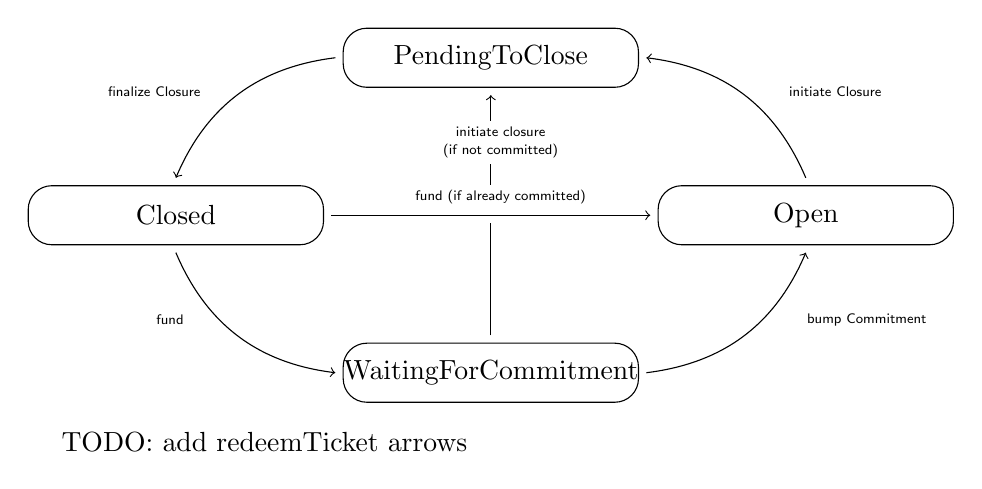
\begin{tikzpicture}[every text node part/.style={align=center}]
        \def\nodeWidth{3.75}
        \def\nodeHeight{0.75}
        \def\padding{0.1}
        \foreach \posX\posY\tag in{0/0/Closed,4/2/PendingToClose,8/0/Open,4/-2/WaitingForCommitment} {
                \draw[rounded corners=3mm,shift={(\posX,\posY)}] (0,0) rectangle (\nodeWidth,\nodeHeight) node[midway] {\smaller{\tag}};
            }

        % Finalize closure
        \draw[->] (4-\padding,2+\nodeHeight/2) to [bend right] (\nodeWidth/2,\nodeHeight+\padding);
        \draw (1.6,1.95) node {\tiny{\textsf{finalize Closure}}};

        % Initiate closure
        \draw[->] (8+\nodeWidth/2,\nodeHeight+\padding) to [bend right] (4+\nodeWidth+\padding,2+\nodeHeight/2);
        \draw (10.25,1.95) node {\tiny{\textsf{initiate Closure}}};

        % Fund
        \draw[->] (\nodeWidth/2,0-\padding) to [bend right] (4-\padding,-2+\nodeHeight/2);
        \draw (1.8,-0.95) node {\tiny{\textsf{fund}}};

        % Bump commitment
        \draw[->] (4+\nodeWidth+\padding,-2+\nodeHeight/2) to [bend right] (8+\nodeWidth/2,0-\padding) ;
        \draw (10.65,-0.95) node {\tiny{\textsf{bump Commitment}}};

        % Initiate closure if not committed
        \draw (4+\nodeWidth/2,-2+\nodeHeight+\padding) -- (4+\nodeWidth/2,\nodeHeight/2-\padding);
        \draw[->] (4+\nodeWidth/2,\nodeHeight/2+\padding) -- (4+\nodeWidth/2,2-\padding);
        \draw (6,1.3) node[fill=white,inner sep=2pt] {\tiny{\textsf{\shortstack{initiate closure\\(if not committed)}}}};

        % Fund if committed
        \draw[->] (\nodeWidth+\padding,\nodeHeight/2) -- (8-\padding,\nodeHeight/2);
        \draw (6,0.6) node[fill=white,inner sep=2pt] {\tiny{\textsf{fund (if already committed)}}};
        \draw (3,-2.5) node {TODO: add redeemTicket arrows};
    \end{tikzpicture}
    \caption{Payment channel states and possible state transitions.}
\end{figure}

In rare cases it can happen that a node $n_{open}$ intends to open a payment channel, but $n_{dest}$ does not submit an on-chain commitment. Under this circumstance, $n_{open}$ has the opportunity to immediately turn the channel into \textit{PendingToClose}.

\paragraph{State}

Each channel is assigned a unique identifier, computed from the addresses of $n_{open}$ and $n_{dest}$,

$$ channelId = keccak256 (\ ethAddr(n_{open}) \ || \ ethAddr(n_{dest}) \ ) $$

where $ethAddr$ maps public keys to Ethereum addresses. Note that using this scheme leads to different $channelIds$ for the channel from $n_{open} \rightarrow n_{dest}$ and the one from $n_{dest} \rightarrow n_{open}$.

Once $n_{open}$ locks funds, the smart contract instantiates the data structure \textit{ChannelData} and stores it under the previously computed $channelId$ within its storage. Instantiation of \textit{ChannelData} can happen it two ways: either there has been a previous instance of the channel of not. If there were one, the smart contract keeps the values $commitment$ and $epoch$ from the previous instance. For $epoch$ this is necessary because tickets from previous instances must lose their value once the channel gets closed. This is achieved by incrementing $epoch$ on every incarnation of the channel. On the other hand, commitments are kept to simplify channel reopenings.

\begin{figure}[H]
    \centering
    \begin{tabular}{c|l|c|c|}
        \cline{2-4}
                                                     & \textbf{Value} & \textbf{Ethereum datatype} & \textbf{size (in bytes)} \\
        \cline{2-4}
        \noalign{\smallskip}
        \cline{2-4}
        \multirow{7}{*}{\rotatebox{90}{ChannelData}} & Balance        & uint256                    & 32 bytes                 \\
                                                     & Commitment*    & bytes32                    & 32 bytes                 \\
                                                     & Ticket Epoch   & uint256                    & 32 bytes                 \\
                                                     & Ticket Index   & uint256                    & 32 bytes                 \\
                                                     & Status         & enum                       & 32 bytes                 \\
                                                     & Epoch*         & uint256                    & 1 bytes                  \\
                                                     & Closure Time   & uint32                     & 4 bytes                  \\
        \cline{2-4}
    \end{tabular}
    \caption{The structure of a stored channel. Values marked with * survive reincarnations of the channel.}
    \label{fig:channeldata}
\end{figure}

Closing a channel sets $closureTime$ to current UNIX timestamp plus the timeframe\footnote{As of now, the timeframe is set for debugging purposes to five minutes.} in miliseconds in which node $n_{dest}$ is allowed to submit previously unredeemed tickets.

\begin{comment}
\paragraph{Opening a channel} Node $A$ can open a channel by transferring funds to the payment channels contract \textit{HoprChannels} and including the following \textit{userdata}:

$$[A: address, B: address, \lambda: uint8, \mu: uint8], \mu = 0,$$

where $\lambda$ is the amount to be staked by $A$. This call will trigger an on-chain event \textit{ChannelFunded} and open a unidirectional payment channel from $A$ to $B$. The payment channel will start in state \textit{Waiting for commitment}. The destination address of the payment channel must now set an on-chain commitment in order for the payment channel between both parties to become \textit{Open}. This is done by $B$ calling the \textit{bumpChannel()} function to make a new set of commitments towards this payment channel. This call will trigger an on-chain event \textit{ChannelOpened} and bumps the ticket epoch to ensure tickets with the previous epochs are invalidated. Every time the channel changes its state, an on-chain event \textit{ChannelUpdated} is emitted.

\paragraph{Redeeming tickets}
As long as the channel remains open, nodes can claim their incentives for forwarding packets via tickets. Tickets are redeemed by dispatching a \textit{redeemTicket()} call to an \textit{Open} payment channel.

If $B$ tries to redeem a ticket from the channel $A\rightarrow B$ (spending channel), but there is an open channel $B\rightarrow A$ (earning channel), $B$'s rewards will be transferred to $B\rightarrow A$ (earning channel). Otherwise, rewards will be sent directly to $B$.

\paragraph{Closing a channel}
Nodes can close a payment channel in order to access their previously staked funds. Only the payment channel creator can initiate the process by calling \textit{initiateChannelClosure()}. This changes the state to $Pending to close$ and triggers a grace period during which the destination node can redeem any unredeemed tickets. Nodes should actively monitor blockchain events to be aware of this payment channel state change.

Once the grace period has elapsed, the payment channel creator can call \textit{finalizeChannelClosure()} which changes the payment channel to $Closed$. When a payment channel is closed, the remaining funds are automatically transferred to the payment channel creator. The channel epoch increments, meaning any unredeemed tickets can no longer be redeemed.
\end{comment}

